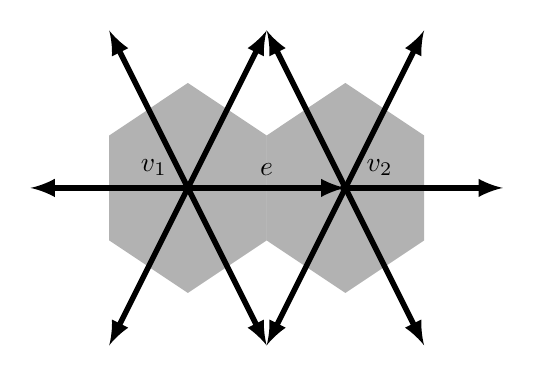
\begin{tikzpicture}[>=latex, line width=2pt, scale=1]
  % Coords
\coordinate (V0) at (0,2);
\coordinate (V1) at (2,2);
\coordinate (V2) at (1,0);
\coordinate (V3) at (1,4);
\coordinate (V4) at (-1,4);
\coordinate (V5) at (-1,0);
\coordinate (V6) at (-2,2);

%circumcenter
\coordinate (CC1) at (1,1.333);
\coordinate (CC0) at (1,2.666);
\coordinate (CC3) at (-1,1.333);
\coordinate (CC2) at (0,0.666);
\coordinate (CC4) at (-1,2.666);
\coordinate (CC5) at (0,3.333);

 % Coords
\coordinate (VS0) at (2,2);
\coordinate (VS1) at (4,2);
\coordinate (VS2) at (3,0);
\coordinate (VS3) at (3,4);
\coordinate (VS4) at (1,4);
\coordinate (VS5) at (1,0);
\coordinate (VS6) at (0,2);

%circumcenter
\coordinate (CCS1) at (3,1.333);
\coordinate (CCS0) at (3,2.666);
\coordinate (CCS3) at (1,1.333);
\coordinate (CCS2) at (2,0.666);
\coordinate (CCS4) at (1,2.666);
\coordinate (CCS5) at (2,3.333);

\fill[black, opacity=0.3] (CC0) -- (CC1) -- (CC2) -- (CC3) -- (CC4) -- (CC5) -- (CC0);
\fill[black, opacity=0.3] (CCS0) -- (CCS1) -- (CCS2) -- (CCS3) -- (CCS4) -- (CCS5) -- (CCS0);

\draw[->](V0) -- (V1) node[midway, above]{$e$};
\draw[->](V0) -- (V2);
\draw[->](V0) -- (V3);
\draw[->](V0) -- (V4);
\draw[->](V0) -- (V5);
\draw[->](V0) -- (V6);

\draw[->](VS0) -- (VS1);
\draw[->](VS0) -- (VS2);
\draw[->](VS0) -- (VS3);
\draw[->](VS0) -- (VS4);
\draw[->](VS0) -- (VS5);
%\draw[->](VS0) -- (VS6);


\fill[] (V0) node[above left] {\(v_1\ \)} circle (2pt);
\fill[] (VS0) node[above right] {\(\ v_2\)} circle (2pt);




\end{tikzpicture}

